\newcommand{\mypath}{../thesis}
\newcommand{\mypathintro}{../thesis/intro}
\chapter{Introduction}
This thesis focuses on reliability issues for the electricity grid that powers the United States.  Electricity is a critical service used by almost every person and company within our country.  Reliability issues cost industry billions of dollars every year.  Large scale power outages are national disasters due to the loss of services such as cell phones, city wide water pumping, gasoline stations, trains, subways, and cooling which inevitably lead to economic loss and loss of life.  

The introduction starts with an overview of the electrical infrastructure of the United States.  Following are the basics of how the power system operates on a day-to-day basis and the organizational structure that operates it. Then, the events of August 2003 are explained where part of the Northeast electricity grid collapsed in a cascading power failure leading to millions of people without power, billions in economic loss and the loss of life.  This is just one example of a large scale power outage, which is rare, but extremely costly to society. After this, general reliability issues of the power grid will be discussed which cost society billions annually.
 
After defining the problem, this thesis explains the tools and methodology for attempting to make our system more robust against such failures.  First, the current literature on cascading power failures is explored.  This is used to model the cascading process as a multi-stage stochastic program with mixed-integer decision variables.  It is shown to have a similar distribution to the simulation, however is computationally difficult.  We turn to optimizing design problems with the cascading simulation as a subproblem.  This allows us to take advantage of accessory information in the cascading simulation as well as parallelize the computational effort to solve large scale problems in  a timely manner.  Finally, a system risk measure is developed to control endogenous, congestion based line failure risk.  This risk measure is used in a real time dispatch model with net injection uncertainty and the cost-risk frontier is explored.

%First, a model of the cascading process is made.  This model captures the effects of the cascading process while remaining simple enough to solve in a reasonable time.  After a model is developed, design problems are formulated in order to improve either the infrastructure or the operation of the system.  These design problems fit into broad families of optimization problems.  Algorithms for these types of problems are used and modified for our particular problem.  Finally, with the help of computation resources, solutions are found to these design problems in order to gain insight into the problem and help protect our system from potential future outages.

\section{Power Systems Introduction}
The United States electrical infrastructure is complex physical structure which connects the consumers of electricity with generating assets over a large geographical area.  The nature of electricity makes the operation of this infrastructure extremely difficult and is accomplished through numerous organizations and people working together to supply electricty at the least cost while maintaining a given level of reliability.

	As of 2004, the electrical infrastructure was comprised of more than \$1 trillion in asset value.  This includes over 200,000 miles of high voltage transmission lines, 950,000 MW of generation, and 3500 utility organizations serving 283 million people.\cite{northeast_2003}  The introduction briefly looks at generation and the transmission system which efficiently moves the energy over long distances.

\subsubsection{Electricity Generation}
	Electricity is generated using a variety of fuels and procceses.  The most common method of electricity generation creates steam by heating water, which spins a turbine producing an alternating current of electricity.  The United States operates its power grid at 60 hz, that is, the direction of electrical flow switches 60 times every second.  Since the generators are tied to the grid, when the grid is stable, the generators are rotating synchronously with the power grid.  The water can be heated by different fuels such as coal, natural gas, fissioning heavy elements such as uranium, or even using geothermal temperature differentials.  The Rankine cycle is a model of converting heat into mechanical energy for steam engines.  The efficiency of the cycle is limited by the difference between the turbine entry temperature and the condenser temperature.  This means that steam cycle power plants need an external cooling source which removes the waste heat from the working fluid before it begins the cycle again.  

	The first example of a steam cycle power plant is a coal plant.  The chemical energy in coal is converted into thermal energy and byproducts such as carbon dioxide.  Power from coal provides around 40\% (for the year 2013 \cite{eia_gov}) of the electricty generation in the United States. These plants have more thermal inertia making changing the output level a slower process.  Modern coal plants achieve efficiencies of 30-40\%, that is the percentage of input energy which is injected into the grid as electricity.

	Nuclear power plants (19\% of electricity) also operate on the steam cycle, producing heat by fissioning heavy elements such as Uranium-235.  Nuclear plants have relatively slow ramping rates and cheap fuel, which lead them to be dispatched at high output rates continuously.  These plants, along with coal plants, provide the majority of baseload power production. Baseload power is the minimum amount of power that needs to be produced continuously throughout the day.  Nuclear fuel has a desirable aspect of being extremely energy dense.  The energy density of Uranium-235 is roughly 3 million times denser than coal.  This means that the waste products of this process are much less than other types of power plants and are also captured completely without being released to the environment.

	Natural gas plants (27\% of electricty) can capture, in addition to the heat energy, the combustion energy and use it to spin a gas turbine.  Gas turbines, while having a lower thermal efficiency, have the desirable trait to quickly throttle production to the desired level in contrast with steam cycles.  Additionally, by using a combination of both combustion and heat energy, combined-cycle natural gas plants can reach efficiencies of around 60\%.  These fast ramping rates and more expensive fuel lead natural gas plants to provide peaking power matching electrical demand over baseload.  Recently, with relatively cheaper natural gas and increased efficiencies from combined-cycle plants, natural gas plants are playing more of a role for electrical demand between baseload and peaking levels.    

	Hydroelectric power (6\% of electricity) has many desirable traits and it is the largest source of renewable energy generation installed around the world.  By creating a reservoir to hold a large amount of water at a high level, potential energy can be stored.  When this water is released, it becomes kinetic energy, which can be captured by a turbine and used to generate electricity.  By controlling the flow into the turbine or the amount of turbines spinning, hydro power is capable of not only storing energy, but also quickly adjusting its output rate.  However, they have the additional constraint of needing to maintain given reservoir levels throughout the year.

	In the past decade, we have introduced a sizeable amount of electricity production from renewable sources such as wind turbines and solar panels (both total 6\% of electricity, with wind comprising the majority).  These generation sources have a cheap fuel (kinetic energy from the wind and solar radiation), but are unable to control output.  

	The different characteristics of generators give them different roles to play in the operation of the power system in order to meet demand.  These various generation assets are owned by utilities, independent power producers, large industrial customers themselves, and, more recently, residential consumers.  

\subsubsection{Transmission Network}
	The production from the majority of large generation plants is at lower voltages (10kV - 25kV).  Electricity traveling in power lines lose energy due to resistive losses, which primarily goes into heating up the power line.  The resistive losses are proportional to the current.  In order to reduce losses, the voltages are stepped up to between 230 kV to 765kV for long distance transmission elements, which has the effect of reducing the current for a given amount of power.  At the demand side, there are radial tree-like distribution networks operating at low voltages (less than 1kV) which connect every demand node to the power grid.  The United States power grid is broken into three distinct power grids: Western Interconnection, Eastern Interconnection, and Texas Interconnection. Each has a network of transmission lines connecting all of the generators with all of the loads.  

	Power flows, according to the laws of physics, along ``paths of least resistance", which are modeled with Kirchoff Voltage Laws (KVL) and Kirchoff Current Laws (KCL).  This means that electricity flow can't be controlled like many other complex networks such as cell phone and internet traffic, but instead follows laws of physics much like water or gas in pipe networks.  In addition, electricity flows at close to the speed of light and currently is hard to store economically, unlike water and gas.   There needs to be an instantaneous balance of generation and demand.  

\subsubsection{Organizational Structure}
The primary reliability organization which develops operating and planning standards is North American Relaibility Council (NERC) and ten regional councils. 
\begin{description}
\item[NERC] develops standards for reliable operation and planning of the bulk electric system and then monitors and assesses compliance.  Also, they provide education and training, while coordinating critical infrastructure protection, such as information exchange between reiliability service organization.  Finally, they assess, analyze, and report performance and system adequacy.
\end{description}
 The primary focus of the relability and planning standards is to be able to serve all demand reliability both today and in the future.  There are 7 primary tasks:
\begin{itemize}
\item Balance power generation and demand continuously;
\item Balance reactive power supply and demand to maintain scheduled voltages;
\item Monitor flows over transmission lines and other facilities to ensure thermal limits not exceeded;
\item Keep system in stable condition;
\item Operate so that it remains in reliable condition even if contingency occurs (N-1 critiera) and when a contingency does occur, maneuver to new stable N-1 position. The N-1 criteria states that the system must be robust against any single component of the power grid failing;
\item Plan, design, and maintain the system to operate reliably; and
\item Prepare for emergencies.
\end{itemize}

Within the United States, Federal Energy Regulatory Commission (FERC) is the federal agency with control over electricity sales, natural gas and oil pipelines, and hydropower projects and has increased power after the  Energy Policy Act of 2005.  This differentiates it from NERC in that it can impose mandatory standards.

\begin{description}
\item[FERC] imposes mandatory reliability standards for the bulk transmission system and imposes penalties on those that manipulate the markets.  Its primary tasks are:
\end{description}
\begin{itemize}
\item Regulate transmission and wholesale electricitity sales in interstate commerce;
\item License non-federal hydroelectric projects;
\item Ensure reliability of high voltage interstate transmission system;
\item Monitor and investigate energy markets;
\item Penalize violating entities, through civil penalties or other mean; and
\item Oversee environmental matters relating to major policy initiatives.
\end{itemize}

The restructuring of the power grid has decoupled utilities from the responsibility of maintaining a control area.  The 140 control areas are operated by the 10 regional Independent System Operators (ISOs) or Regional Transmission Organizations (RTOs).  
\begin{description}
\item[ISO/RTO] are tasked with providing least cost energy to everyone within its territory while maintaining a given level of reliability.  In order to do this, they create wholesale electricity markets in order to balance generation and load in real time at least cost.  Their tasks are:
\end{description}
\begin{itemize}
\item Manage the wholesale electricity markets while maintaining the reliability of the system; 
\item Direct the operation of the assets owned by their members; and
\item Can encompass multiple control areas within the territory that they operate.
\end{itemize}

\subsubsection{Wholesale Electricity Markets}
The ISO or RTO use 3 primary markets for determining how much each generator should produce at any given time.  The first market is bi-lateral contracts.  These are long term contracts between producers and suppliers to exchange a certain quantity of energy at a given price.  These contracts help provide reliable, long term forecasting for supply and load. This reduces exposure to the volatility of the day ahead and real time markets.  

The day ahead market takes bids from generators which contain an array of costs to produce a certain amount of electricity.  The generators also provide additional constraints which they need to operate within, such as ramping rates and start-up and shut-down times and costs.  In addition to generators' physical constraints, forecasts for demand of the following day will be used to get an estimate of the amount of generation needed.  Using the transmission constraints for the given network, the ISO will clear this market during the previous day.  This process usually takes around four hours and is done with specialized optimization tools solving the optimal power flow problem with security constraints and unit commitment decision variables.  The outcome of this process is the schedule for slow ramping generators and hourly locational marginal prices (LMP) at each location in the network for the following day.  These prices are guaranteed and any deviation from the schedule will need to be made up in the real-time market.	

The real-time market makes up for errors in forecasting as well as possible outages in generation or transmission.  This market operates on five minute intervals and can be extremely volatile.  Similar methods are used to clear this market, although simplified due to the time constraint.  Price spikes can occur during times of peak demand and a congested grid in which the price of electricity can often become over 10-20 times as expensive.  The reverse is also possible.  During times of low demand it is possible for negative prices on the real time market.  This occurs because the generators are constrained by ramping rates and there is too much production on the grid. In figure (\ref{fig:lmpmiso}), there are negative prices across the Midwest and, in particular, Iowa, with much higher prices in Illinois.  This LMP snapshot is taken at night when there is low demand for electricity as well as increased production from wind farms located in the Midwest.  The differences in prices suggest transmission constraints between the Upper Midwest and Illinois.   


\begin{figure}
\centering
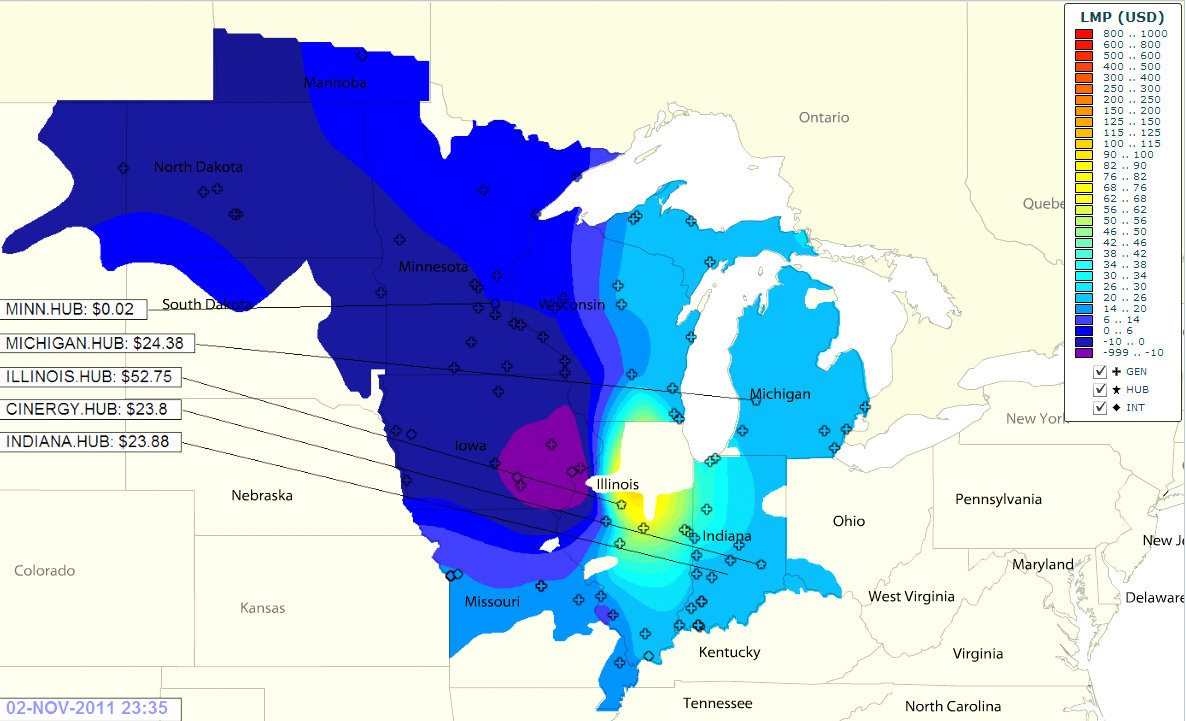
\includegraphics[width=5in]{lmp}  
\caption{Location Marginal Prices (LMP) for Midwest ISO's territory}
\label{fig:lmpmiso}
\end{figure}


\subsubsection{Operating Constraints}

In order for the power grid to operate and maintain stability, a number of things must hold.  First and foremost, there must be a continuous balance of power generation and demand.  The US grids are all operated with a target frequency of 60 hz, but the actual system frequency varies.  When there is excess generation on the grid, the frequency will increase and with a lack of generation, frequency will drop.  Since the generators are synchronized with the grid, when the frequency deviates from normal, the generators can move out of their operating limits and cause damage.  Generators will have internal protections to identify bad operating points and trip offline in order to protect themselves.  In order to protect the grid, there is automated tripping of load at certain frequency points to take customers off line and prevent total collapse.  

In addition to real power balance, reactive power supply and demand must be used to maintain scheduled voltages.  Low voltage can cause system instability and damage to motors and electrical equipment.  Also, high voltage can exceed insulation capability and cause dangerous arcs.  Reactive power is supplied through capacitor banks and generator output.

In order to protect the transmission elements, the flows over transmission lines and other facilities must be monitored to ensure thermal limits are not exceeded.  Lines are heated by electricity flow and equipment can be damaged, such as conductors sagging from stretch and expansion due to high temperatures.  These problems are affected by ambient temperature and wind conditions.  The flow is limited so the line does not sag into obstructions such as trees and telephones.



\section{Cascading Power Failures}
A cascading power failure is a set of failures of individual components of the transmission system which leads to the redistribution of power over the new topology.
 When the system is in a stable operating position, individual components will often have a negligable effect on system-wide distribution.  However, after several failures, the transmission network may not have enough capacity to distribute the power from the generation to the load.  This can cause a series of fast acting trips in which a large portion of the grid may fail.  While rare, these events are extremely costly.


\subsection{Northeast 2003 Blackout} 

%This account of the Northeast Blackout is drawn from the \textit{Final Report on the August 14, 2003 Blackout in the United States and Canada} by the U.S.-Canada Power System Outage Task Force.\cite{northeast_2003}  

\subsubsection{Historical Problems}
The Northeast blackout of 2003 began in the Cleveland-Akron area of the Eastern Interconnection.  This area had a history of problems of low voltages due to the relatively high amount of imported power.  In 1998, the system was becoming unstable and everything other than load shed was done to fix the problem.  It was shown to not be within the reliability standards, and regulations were loosened instead of addressing the problem.  A transformer problem led American Electric Power (AEP), a control area entity, to perform a reliability study on the neighboring control area operated by First Energy (FE).  The study again showed voltage instability problems.

The summer of 2003 was fairly typical with less than historical peak load.  While the load was less than historal peak, it was consistently greater than the forecasted load.  High temperatures, creating a greater air conditioning load, contributed to reactive power shortages.  The voltages were low in Cleveland-Akron during the week, but within the new operating limits (92\% to 105\%).  A group of shunt capacitors, out of service for planned maintenance, further reduce reactive power supply.  Also, a large nuclear reactor, Davis-Besse, was in a long term forced outage state.  This plant is normally able to provide a large amount of real power as well as reactive power support.

\subsubsection{Normal Day Turns Bad}
A series of initiating events, as well as the failure of FE's control server, led to an unstable system and the inability for operators to do anything about it.  In addition, neighboring regional reliability coordinators (Midwest Independent System Operator, MISO, and Pennsylvania-New Jersey-Maryland Interconnect, PJM) had bad information on the state of the system and were unable to provide support.  The operators had concern about voltage levels and were trying to get additional reactive power online.  The shunt capacitors were unable to return to operation.

The following initiating events didn't cause the system to collapse, but moved it into an unreliable state, which allowed the collapse to take place. The Stuart-Atlanta 345 kV line tripped due to contact with surrounding vegetation (area voltage at 98.5\%) at less than 100\% capacity.  In addition to the loss of the line, MISO was unaware, which led to unusable output and the inability to provide support.  An important generating unit, Eastlake 5, attempts to increase reactive power output, but the internal protection trips the generator offline (area voltage 97.3\%).  This led to real power imports rising, which increased the need for reactive power as well.  Another transmission line loss of Harding-Chamberlin 345 kV continued to depress the voltage (95.9\%).  Around this time, the underlying 138 kV network began to fail.   MISO was unable to perform N-1 contingency analysis and the FE reliability charts flatlined due to the server problems.

Ultimately, it was in reliable state before 15:05, however, after all of these events, the system was no longer N-1 stable.  In addition, reliability coordinators were using separate state information due to poor communication.  

\subsubsection{System Becomes Unreliable}

A total of 3 lines tripped at below operating capacity due to tree contact starting with Harding-Chamberlin (44\% of capacity) at 15:05.  Then the Hanna-Juniper line tripped (88\% normal and emergency rating) at 15:32.  The Star-South Canton line had multiple tree contacts (55\%) starting at 14:27, and finally tripped off for good (93\% emergency rating)  at 15:41.  There was no prior sustained outages from tree contact in the previous years and FE used vegetation management practices consistent with the industry.  When designing line limits, the thermal ratings are based on many variables including ambient temperatures and wind speeds.  A combination of higher than nominal ambient temperature and lower wind speeds reduced the cooling capacity of lines.

Perry plant, the largest local generator, was getting voltage spikes at levels close to tripping the generator.  They notified FE of the problems, but the operators were unable to recover from this precarious situation.  The task force notes that load shed here of 1500MW may have saved the system by increasing voltages and stopping the ultimate trip of Sammis Star line.

\subsubsection{High Speed Cascading Failures}
At 16:05 the final straw was pulled by the tripping of the Sammis-Star 345kV line seperating geographical regions of the grid.  Unplanned power shifts across regions caused phase 3 operations, which trip lines far away from the problem area.  The grid continued to stabilize after each one of these individual outages.  However, by 16:10, the north and south separated (AEP separates from FE), and the high generation area was no longer directly connected to the high load center.  This caused a massive power surge from PJM through New York and Ontario counter clockwise around the great lake to load centers in Michigan. This surge caused the Northeast to separate from the rest of Eastern Interconnect (EI).

There was insufficient generation in the newly formed islands to support the load.  The frequency in remaining parts of EI rose to 60.3\%, representing 3700 MW of excess generation.  The Northeast grid kept breaking apart until islands were formed in which an equillibrium between load and generation could be made.  Under-frequency and under-voltage load shedding helped to stabilize the system within the islands.  New York dropped 10,648 MW through automatic load shedding and Ontario dropped 7800 MW.  Some generators tripped off at unreasonable levels making island stabilization more difficult.  Thousands of events occured between 16:10 and 16:13.  

The cascade spread, not due to voltage problems, but dyanmic power swings which caused system instability.  The voltage instability was only companion to the angle instability (represents large real power flow swings) which tripped generators and lines.  The large power swings come from imbalance between generation and load across regions and the electrical separation of these two areas.  The inherent weak points are lines with the highest impedence, which trip off relatively early due to protective relay settings.  These are typically long over-head lines with high loadings.


\subsubsection{The Blackout Results}
In the United States, 45 million people lost power totaling 61,800 MW in Ohio, Michigan, Pennsylvania, New York, Vermont, Massachusetts, Connecticut, and New Jersey.  The US loss estimate was between \$4 billion and \$10 billion.  Another 10 million people from Canada lost power leading to an estimated 18.9 million lost man hours and \$2.3 billion in lost manufacturing shipments.   There were at least 11 fatalities, power took up to 4 days to return, and rolling blackouts continued in Ontario for the following week.\cite{northeast_2003}

The formation of a large island, based off of hydro plants in western New York and Canada, was the basis for system restoration.
 

\section{Reliability in Power Systems}
The electricity grid is held to a higher reliability standard than other services since it is critical infrastructure for society.  Even though the power system maintains a very high level of reliability, power interuptions still have large costs to consumers.  After a discussion of the economic costs, the trends in power outages for the North American grid will be looked at.

The economic loss caused by power interruptions to electricity consumers in the United States for 2001 was estimated at \$79 billion.\cite{lacommare_2006}  This can be compared to the total revenue of electrical sales in the year 2001 of \$247 billion.\cite{eia_sales}  The single event of the Northeast blackout in 2003 was estimated to have a total impact on US workers, consumers, and taxpayers as a loss of approximately \$6.4 billion.\cite{anderson_2003}  This cost is hidden from the system, but may entertain the notion that the true cost of electricity is higher than the current prices.  

The current power system has evolved throughout the last century due to economic and reliability issues and the responses of the operating entities to these forces.  The power system has self-organized into a dynamic equilibrium where blackouts of all sizes occur \cite{dobson_2001}.  The average frequency of blackouts in the United States is 13 days and has been the same for 30 years \cite{carreras_2004}, which represents this equilibrium.  
	
NERC data shows that distribution of blackouts for the last 15 years (1988-2003) follows a power tail curve with an exponent of around $-1.3\pm.2$ \cite{carreras_2004}. This is strengthened further where Hines et. al. showed that show the frequency of blackouts in the United States is not decreasing, changes seasonally and with the time of day, and follows a power-law distribution.\cite{hines_2008} \cite{hines_2009}

Some emerging conditions on the grid may make protection more important and more difficult (table \ref{tab:change1}).  Electric vehicles adopted in masse have a potential to offer useful services to the power grid through the use of a sizeable amount of energy storage in aggregate.  However, they also represent a considerable stress on the system in different spots and ways than it is used to.  The ideal car battery system would have a quick charge, that is, the ability to transfer the energy from the grid to the battery extremely quickly.  This would allow consumers to use charging stations similar to the current gasoline stations for combustion engines.  A charging station capable of charging many cars would have extremely high and unpredictable volatility that the system will need to protect against.

The increased penetration of renewable energy production also increases stress on the power system.  Wind and solar are both variable generation devices which do not actively control the amount of electricity being produced.  The system needs to maintain ample ramping capability in order to maintain stability.  These stresses can be reduced by improving the quality of forecasting efforts on various timescales.  In addition, these technologies are geographically constrained by their fuel source availability, wind speeds and solar irradition.  However, these natural fuel sources do not align with large demand centers, so the transmission system is needed to efficiently distribute the energy produced.

\begin{table}
\centering
\footnotesize
\begin{tabular}{| p{7cm} | p{7cm} |}
\hline
\bf Previous Conditions 	&	\bf Emerging Conditions 		\\	\hline  	\hline
Fewer, relatively large resources	&	Smaller, more numerous resources		\\	\hline
Long-term, firm contracts 	&	Contracts shorter in duration, more non-firm transactions, fewer long-term firm transactions	\\	\hline
Bulk power transactions relatively stable and predictable	&	Bulk power transactions relatively variable and less predictable	\\	\hline
Assessment of system reliability made from stable base (narrower, more predictable range of potential operating states)	&	Assessment of system reliability made from variable base (wider, less predicatable range of potential operating states)		\\		\hline
Limited and knowledgable set of utility players 	&	More players making more transactions, some with less interconnected operation experience; increasing with retail access	\\	\hline
Unused transmission capacity and high security margins	&	High transmission utilization and operation closer to security limits	\\	\hline
Limited competition, little incentive for reducing reliability investments	&	Utilities less willing to make investments in transmission reliability that do not increase revenues	\\	\hline
Market rules and reliability rules developed together	&	Market rules undergoing transition, reliability rules developed separately	\\	\hline
Limited wheeling	&	More system throughput	\\	\hline
\end{tabular}
\caption{\small Changing conditions that affect system reliability (from the Northeast outage report \cite{northeast_2003}).}
 \label{tab:change1}
\end{table}

\section{Thesis Roadmap}
Ultimately, we need to be able to give operators good information and as much time as possible to be able to react to the contingency and avert collapse.  In order to give the operators more time, we must make the system more robust to contingencies.  To this end, we develop a method to efficiently optimize design problems with cascading failures as subproblems.  Additionally, we formulate a new dispatch model which controls system risk explicitly.

\subsubsection{Multi-Stage Integer Program}
The first chapter gives an overview of current literature on cascading power failures.  This process is then modeled as a multi-stage stochastic program with mixed integer decision variables (formulation donated as MSIP).  The primary contributions of this chapter are:
\begin{itemize}
\item Describe sequential cascading process and its greedy characteristics mathematically
\item Model decision dependent uncertainty using binary variables and a priori sampling using concept of effective capacity
\item Formulate cascading simulation as MSIP and use as subproblem in long-term design optimization
\end{itemize}

\subsubsection{Derivative Free Optimization}
The second chapter uses the computationally cheaper simulation, common random numbers for variance reduction, and parallelization to optimize design problems using the cascading (OPA) simulation as a subproblem.  To optimize over this simulation with high frequency noise and discontinuities, derivative free optimization (DFO) techniques were employed.  The primary contributions of this chapter are:
\bi
\item Extend cascading analysis from sensitivity analysis to full optimization
\item Efficient parallel implementation to optimize simulation over large scale instances
\item Modify DFO techniques to take advantage of problem specific characteristics while maintaining local convergence guarantees
\ei

\subsubsection{Joint Chance Constraint}
The third chapter works to change the market model to incorporate the endogenous risk from line loading.  A system risk measure is modeled as a joint chance constraint (JCC) on the probability of any line failing and constrained under net injection uncertainty.  The primary contributions of this chapter are:
\bi
\item System risk formulated analytically as a JCC using mean branch flow and branch covariance matrix
\item Risk measure allows the ordering of different dispatch points with respect to line loading characteristics
\item The cost-risk frontier is explored under this new risk measure and the economic trade-offs explored
\item System risk measure is extended to exogenous contingencies and reliability is evaluated using the OPA model
\ei

\subsection{Overview}
\subsubsection{Cascading Power Failures}
The topological model of the power grid is composed of the various elements in the transmission network as well as their parameters.  While these types of models are simple, they are incapable of capturing effects which are loading dependent. The OPA type model (detailed in section \ref{opa_section}) is a sequential process in which the power flows for the entire network are calculated in order to determine the loading on the various transmission elements.  This in addition to a deterministic or probablistic failure model is used to outage individual components at each stage in the cascade.  The cascade concludes when no elements are outaged.

Even in its simplest form, this OPA type of model has been shown to capture the criticality effects of blackouts (higher than expected large blackouts) we see in real power systems in aggregate.  As more complexity is added into this model, this type of model can produce reasonable sequences of outages for the system, while remaining accurate in aggregate. 

Building this model requires calculating the power flows.  While the system is not necessarily stable or balanced throughout the cascade process, the balanced, steady state 3 phase power flow equations will be used as a basis for the power flow analysis.  This keeps the calculations tractable and gives valuable information about the various topologies and loading patterns.  In the simplest form of the OPA Model, the power flows will be approximated using the DC (Decoupled) power flow model, which is a linear approximation to the AC power flow equations.


Design problems will be formed that change aspects of the topology, component parameters, or operation of the system.  Using the OPA model to gauge the response of the system to these changes, we will have formulated a mathematical optimization problem.  These design problems can range from transmission expansions to setting operational reserve levels or even producing protective relay settings for individual components.

%In addition to the OPA model, accessory information can be used to aid in the optimization process.  This includes things such as pseudo-topological statistics (electrical distances and centrality), line outage patterns and recognition, and finally, economic information.  Additionally, making a link between reliability and economics use of an economic dispatch model.
\subsubsection{Optimization Difficulties}
This problem offers several difficulties which make optimization challenging.  

A primary difficulty is the sequential process of the OPA model in which operators make decisions under uncertainty and the decisions effect the future stages and progression of the process.  In addition, the decision dependent outcomes only have a probabilistic effect on the progression of the cascade.  That is, an overloaded line may not fail in all scenarios, so that at each stage a range of outcomes is needed to capture the probabilistic effects.  In order to properly describe the outcomes of the process under a range of scenarios, a multi-stage tree with even a modest number of stages and outcomes explodes quickly.

Another main challenge is that the change of topology of the power system creates nonlinear and nonconvex effects.  It is possible to reduce the cost of electricity by removing transmission elements.  On the other hand, by adding transmission lines, a system capable of meeting demand can become infeasible.  Since the system is constrained by KVL and KCL, each transmission line, while providing a path for electricity flow, further constrains the system.  It is well known that nonconvex behavior is not desirable for optimization problems, and in this case we can have nonconvex behavior between each stage of our process, since by definition, each stage before the final has topology changes.

\subsubsection{Modeling Cascading Power Failures}
In order to better understand the structure of the problem, it will be formulated as a multi-stage stochastic program with decision-dependent uncertainty (MSIP).  In order to do this, logical connections between the stages will be made using binary variables, that is variables that can only take the value 0 or 1.  In this way, the decision dependent uncertainty can be modeled explicitly and the probalistic effects can be modeled by sampling the random variables a prior.  As the number of outcomes per stage increases, the better the probablistic effects can be modeled.  Using this type of model, the number of stages has to be decided a prior as well.  This is a major shortcoming, as we are concerned with the effects of the worst cascades, which can take many stages to complete.  As the number of nodes, $N$, is related to the number of outcomes, $a$, and number of stages, $b$, by $N \propto a^{b}$, the model quickly becomes intractable. 

 However, if a crude approximation to the cascade process can get similar aggregate effects from the outcome, we will be able to use this formulation as a subproblem.  This can then be embedded in design master problem, an example being transmission expansion, and then solved with an out of the box mixed-integer solver.

\subsubsection{Optimizing Design Problems}
The computational complexity of the first approach grows too fast with respect to increases in model accuracy.  In this approach, the OPA model will be simulated instead of more rigoroursly mathematically defined.  In this we lose some structure of the problem but by decoupling the stages of the OPA model from the master problem, we have a fairly simple monte carlo simulation.  Using variance reduction techniques of common random numbers we can resolve the outcome of any configuration of the design problems extremely quickly by running a large number of simulations.  In addition, we can parallelize the process in order to evaluate multiple configurations simultaneously.  The outcome of these simulations will be statistics about the magnitude of the blackout for the various contingencies as well as possible sequence of outages.

The optimization field has many algorithms that can use a zeroth order oracle, that is for each configuration the oracle returns a real valued number and may include stochastic variation or numerical error.  In our case the simulation is the oracle and the real valued number could be the expected load shed or the value-at-risk which attempts to capture large tail effects of distributions.  The main types of derivative free optimization are pattern search, model based, and stochastic approximations.  

A pattern search method doesn't attempt to understand anything about the underlying structure but instead tries to search in a specific way such that the function value improves.  Certain patterns can offer local convergences guarantees, that is the solution is at least better than all of those in the neighborhood.  This, in combination with a grid search in which the whole space is partitioned and sampled, can get you good global solutions, but global convergence will not be provable.  These search methods can be improved by using well positioned exploratory steps and search directions that conform to local topology.

%  The model based method takes a set of sampled points and builds a polynomial model, typically linear or quadratic, and then optimizes this model exactly.  This type of model can have faster local convergence properties, although in some cases it performs much worse than even a simple pattern search.
%Stochastic models assume an underlying probability distribution about the function.  In addition, assumptions are made such that by increasing sampling infinitely, the sample approximation converges to the true value.  These models can have characteristics of both pattern search and model based methods, but under the assumption of some stochastic error being present.

\subsubsection{Risk Model for Real-Time Dispatch}
The last chapter finishes by considering a new market model for real-time dispatch.  This model incorporates endogenous line loading risk and constrains it according to some risk preference.  This creates an efficient operating frontier along the cost-risk metrics for different operating points.  In addition, this model incorporates net injection uncertainty into the evaluation of the system risk measure.  Included in the system risk measure is the covariance of the net injection uncertainty.  This uncertainty is responsible for some of the system stress due to volatile injection.  With it's explicit representation, we can finally price these stressful assets directly.\endnote{\textbf{Market Model Shortcomings}

The market model should put a price on destabilizing effects.  In order to illustrate some of the shortcomings of the current market, two examples will be used.  The first example will look at generators and highlight the fact that they are not getting paid according to their value to the system.  The second will look at demand and highlight that all demands are not equal and thus should not pay the same marginal price.

The first example is of 2 generators at the same bus of a power system and they have equal marginal cost at some point in time.  Generator A is outputting at its maximum output level but generator B is below its maximum output level.  Generator A is only able to ramp down but generator B is able to ramp up or ramp down.  Generator B provides additional flexibility to the system in order to find a least cost power flow and also increase stability of the system.  In today's market, this generator could bid this capacity into regulation services and get paid.  However, if these generators are not used for ancillary services, they get paid at an equal rate despite offering unequal services.   Furthermore, the regulation and reserve markets are set up so that you can bid into the markets as long as you meet some minimum requirements.  This puts unequal services on the same level and when you are finding a least cost solution, you are likely to deploy inferior quality services.  The market should be able to place the correct value on the true varying levels of service.

The second example is of two different demand profiles at the same node and their demand does not affect the locational marginal price (LMP).  Demand A is a fixed demand and doesn't fluctuate at all.  Demand B has an average demand equal to demand A, but half the time is at twice A's level and half the time at 0.  Since they both consume the same amount of power, these demands both pay the same rate.  But these demands place unequal stress on the system.  If all demand was type B, additional resources would need to be put on the grid to meet demand.  Type B demand also increases the regulation needed to ensure reliability of the grid.  Currently, the regulation services bought to support type B demand is paid for by all demand equally.  The market should be able to place the correct price on the varying levels of stress demand puts on the grid.     

The market model needs to account for the cost of volatility to the system.  Currently, this cost is socialized to the whole system through the cost of ancillary services such as reserves and regulation support instead of being bore by those that cause the instabilities.  In order to properly account for these costs and reward those offering these services, a new market model will be made.  The strengths and weakness of this model will be showed, in particular the effects it has on the likelihood of  cascading power failures.

%A key tool in building the market model will be critical points. The reliability of the electricity grid can be controlled by varying the distance between the operating positions and various critical points.  Using a list of contingencies, costs associated with each contingency can be measured by its new distance to bad operating points.  Once we have a measure, we will have a value to place on entities causing stress to the system and reward those providing the services.  This market will be able to take over both the regulation and reserve markets.  Regulation and reserve markets are incapable of properly pricing reliability issues, which is exactly what they are designed to do.  Instead, due to having set points for how much reserve and regulation they have, there is no ability to toggle how reliable the system is.  However, we know that the reliability of power systems fluctuates seasonally and daily, but the level of support the system is getting is not.  In addition, with the ability to have a tangible measure for reliability, the consumers of electricity will have a better quality product.  The power systems will now have the ability to adjust the cost of electricity for a trade-off in reliability.  This will link the economic and reliability issues of the power grid.  It will allow a uniform system to apply to various tough problems in electricity markets such as demand response and energy storage.

%If we look at an uncertain demand and note it has some average consumption rate over a time interval and a certain amount of variance from its mean, we can see that a load with zero variance will be the cheapest possible load.  Any positive amount of variance will move the system closer to critical points at some point in time over the given interval.  Loads with extremely high variance will have to pay even more as they will move the system even closer to the bad operating points.  Energy storage devices and demand response will be able to play an important role in these markets as well.  It is unlikely that we stumbled onto the reliability frontier and this model should help the system move closer.  

}

We begin by modeling the net injections as a gaussian distribution with a given mean and covariance matrix.  Due to our linear assumptions for DC power flow, the linear power transfer distribution matrix can be used to calculate the branch flows (also gaussian) mean and the branch covariance matrix.  A line failure function is used to model the risk on a single line for a given flow.  This can be integrated over the uncertainty in line flow to find the individual contribution of risk for any line.  By summing over the lines, we find the expected risk to the system depending on the specific line loadings.  This system risk is constrained in a real time dispatch model.

The JCC model is explored for its effects on the generator dispatch points in a small 30 bus example. The model is also used on a 2300 bus example to show that it is quick to solve (around 2-4x solve times compared to standard DC, although roughly similar as standard chance constraint model).  The cost risk frontier is explored and the chance constraint frontier is plotted, which resides on the interior of the new frontier.  The chance constraint model comes from several papers in this research area and puts a chance constraint on the probability of a line to exceed its threshold.  With proper parameters, the JCC model can closely represent the same effects as the chance constraint model while having the additional benefit of a system risk measure, instead of a risk measure for every single branch element.

Finally, the injection covariance matrix will be priced using shadow prices for system risk constraints and carrying through the analytic formulation.  In addition, the system risk measure is extended to exogenous contingencies (N-1 in particular) and the reliability of the system is measured using the OPA simulation.
